\documentclass[hidelinks,10pt]{article}

% PACKAGES

\usepackage{geometry}          % See geometry.pdf to learn the layout options. There are lots.
%\usepackage{harvard}
\usepackage{natbib}

\geometry{letterpaper}                   % ... or a4paper or a5paper or ...
%\geometry{landscape}                % Activate for for rotated page geometry
%\usepackage[parfill]{parskip}    % Activate to begin paragraphs with an empty line rather than an indent
\usepackage{graphicx}
\usepackage{amsmath}

\usepackage{caption}
\usepackage{subcaption}

\usepackage{etoolbox}





\usepackage{lscape}
\usepackage{dcolumn}

\usepackage{color}
\usepackage{longtable}
\usepackage{bbding}
\usepackage{wasysym}
\usepackage{manfnt}
%\usepackage{hyperref}
\usepackage[utf8]{inputenc}
\usepackage[colorlinks=true,allcolors=blue]{hyperref}
%\hypersetup{colorlinks=true,linkcolor=blue, linktocpage}


%\usepackage{geometry}          % See geometry.pdf to learn the layout options. There are lots.
%\geometry{letterpaper}                   % ... or a4paper or a5paper or ...
\usepackage[capposition=top]{floatrow}

\usepackage{amssymb}
\usepackage{epstopdf}
\usepackage{booktabs}
\usepackage{ctable}
\usepackage{threeparttable}
\usepackage{environ}
%\usepackage{threeparttablex}
\usepackage[bottom]{footmisc}
\usepackage{fontawesome}



\linespread{1.3}




\title{COVID-19 in Mexico: Predicting severe disease outcomes using health and socioeconomic variables.\\
\large University of Chicago\\
CAPP 30254: Machine Learning for Public Policy}

\author{Roberto Barroso Luque\footnote{barrosoluquer@uchicago.edu} \and Oscar E. Noriega Villarreal\footnote{onoriega@uchicago.edu} \and Jesica María Ramírez Toscano\footnote{jramireztoscano@uchicago.edu}\and Luz Stephanie Ramos Gómez\footnote{stephanieramos@uchicago.edu}}





\begin{document}
	\maketitle
		\begin{center}
		\faGithub\href{https://github.com/ml-project-2020}{ GitHub Project Repository}
	\end{center}
	


	
	\pagebreak
	
	%\begin{abstract}
			\section{Executive Summary}
		The current pandemic caused by the SARS-CoV-2 (COVID-19) virus represents an unprecedented challenge to the global economy. In order to provide data-driven policy advice to individual countries, analysis and modeling should be done on national-level data. With under-funded healthcare systems, institutional-weakness, and large informal economic sectors, Mexico faces a gigantic challenge to contain the virus. We trained classification algorithms to predict death and hospitalization among individuals who tested positive for the virus in Mexican soil using a mix of health and socioeconomic variables at the individual and municipality levels. \\Using ten-fold cross-validation, linear support vectors, logistic regression, decision trees, and random forest models were trained to predict patient outcomes (survival vs death and hospitalization vs home recovery). In both classification problems, recall was used as the main evaluation metric in order to minimize false negatives. The best models achieved accuracy scores of more than seventy percent and recall scores of more than eighty percent. Feature importance for the optimum models were then analyzed. Age and comorbidities such as diabetes, immuno-suppresion and obesity gave strong predictive power to both COVID-19 death and hospitalization predictions. Surprisingly, health resource indicators such as number of doctors, nurses and hospital beds per 10,000 residents as well as municipality poverty level featured among the top predictors for hospitalization but not for death prediction. A relative risk profile was then constructed from the classification results. \\Our work shows that, despite inaccuracies in governmental data, machine learning can provide insights into important risk factors that may be used to forecast severity of COVID-19 outcomes at the individual level while informing policy at the state level. 
		
		
	%\end{abstract}
	
	%%%%%%%%%%%%%%%%%%%%%%%
	
	\section{Background: COVID-19 in Mexico}\label{sec_context}
	
	Following a now-familiar trend, Mexican authorities, fell prey to excessive hubris as the coronavirus started to spread around the world. 
	In late January, official communication from the Ministry of Health downplayed the risks presented to the Mexican population by the quickly spreading virus\footnote{\href{https://www.reporteindigo.com/piensa/el-nuevo-virus-coronavirus-no-representa-un-peligro-para-mexico/}{\textit{New virus doesn't represent a danger for Mexico.}} José Pablo Espíndola. Reporte Indigo.}. By the end of February, Mexico reported its first official Coronavirus cases: one in Mexico City and one in the northern state of Sinaloa. Despite the alarming pace of global transmission, and the mounting death toll in countries like Italy and Spain, by late March the Mexican government continued with its cavalier attitude\footnote{\href{https://www.brookings.edu/blog/order-from-chaos/2020/03/30/amlos-feeble-response-to-covid-19-in-mexico/}{\textit{AMLO’s feeble response to COVID-19 in Mexico.}} Vanda Felbab Brown. Brookings.}. \\
	As of June 2020, Mexico has over 120,000 official cases and more than 14,000 deaths from the virus. Whether the disturbing state of the pandemic currently unfolding in Mexico is a direct consequence of official government policies or reckless rhetoric from political leaders is a question for academic debate and political punditry\footnote{\href{https://www.thelancet.com/journals/lancet/article/PIIS0140-6736(20)31198-3/fulltext}{\textit{Mexican President López Obrador draws doctors’ ire.}} David Agren. The Lancet.}. Nonetheless, what is abundantly clear from official data is that Mexico has not managed to control the epidemic or ‘flatten the curve’ (Supplementary Figure~\ref{fig:1}).\\
	Official cases, hospitalizations, and deaths as a result of the novel coronavirus continue to rise across the country. Most alarmingly, the country has an average death rate of more than 11\% according to official counts which are substantially larger when compared to similar countries such as Peru (2.8\%), Colombia (3\%), and Brazil (5\%). Mexico’s excessive official death rate could be the cause of low testing capacity, as of June 2020 the country’s testing rate falls at a meager 2,800 tests per million residents, Brazil which is one of the worst-hit countries has a test rate of about double that of Mexico\footnote{ See \href{https://www.statista.com/statistics/1104645/covid19-testing-rate-select-countries-worldwide/}{Statista} data}. Yet until the testing capacity increases the true gravity of the situation will remain unknown. \\
	The severity of the pandemic has not been uniformly felt across the country with the northern states of Baja California and Sinaloa and southern Quintana Roo being particularly hard hit (Supplementary Figure~\ref{fig:2}). Furthermore, as has been the case in most countries, specific segments of the population have been at much higher risk of developing severe outcomes of the disease, with older cohorts and people with comorbidities at much higher risk of dying or being hospitalized as a result of the virus (Supplementary Figure~\ref{fig:3}).\\
Unfortunately, while social isolation measures stem the spread of the virus they also have a devastating economic effect.  Countries, such as Canada and the US have provided emergency funds to help middle- and low-income households through social protection mechanisms. In contrast,  Mexico’s fiscal response has been timid at best and non-existent at worst. With at least half of the labor population in the informal sector  (meaning no access to social protection and/or financial institutions) Mexico’s economy is at a particular perilous state, where Banxico,
Mexico's Central Bank, anticipates a GDP decline of up to 8.8\%\footnote{\href{https://www.banxico.org.mx/publicaciones-y-prensa/informes-trimestrales/\%7B23C2DCA8-4AD3-FBE0-B0BF-4D30C8066B84\%7D.pdf}{\textit{Quarterly Report, January-March 2020}}- Banco de Mexico} in a worst-case-scenario, while private institutions such as Credit Suisse expect a drop of 9.6\%\footnote{\href{https://www.forbes.com.mx/economia-pib-mexico-tendra-peor-caida-1932-credit-suisse/}{\textit{Mexico's GDP will have its worst decline since 1932: Credit Suisse}} - Forbes Mexico, 04/30/2020} in GDP. Given its limited resources, it is of imperative importance that the Mexican government prioritize the most vulnerable areas and allocates resources accordingly.\\
However, due to a lack of research and analysis, it is far from clear which states and municipalities are most at risk. To address this analysis gap we analyzed official COVID-19 cases provided by the Ministry of Health and complemented this data with health resources, demographic, and poverty data at the municipality level from several public sources. We trained classification algorithms on health and socioeconomic variables to predict the severity of COVID-19 outcomes and used our result to develop a relative risk profile for all Mexican states. We hope that this work can serve to inform Mexican politicians and policy leaders so that they can provide data-driven solutions to the current crisis. Furthermore, we hope our analysis will prove useful to the Mexican research and scientific communities so that they continue to work on investigating and understanding the nature of the pandemic in our country.

	\section{Data}\label{sec_data}
	
	The data used for this analysis is all publicly available and can be accessed online through several governmental institutions. The relevant unit of observation in our work is the individual, nonetheless, due to the relevance of location level information we complemented individual level data with municipality level information relevant to each individual in our data set. In particular, we used information of the available health infrastructure at the municipality level as a proxy for health/medical resource availability. \\
	Individual level data used in this analysis came from daily COVID-19 reports made available by the Mexican Federal Health Ministry (SSA). This dataset\footnote{\href{http://187.191.75.115/gobmx/salud/datos_abiertos/datos_abiertos_covid19.zip}{\textit{ datos.gob.mx COVID-19 Open Data}}} contains information on all administered COVID-19 tests in Mexico, including characteristics of the individual tested such as age, sex and location where the test was administered. Furthermore, this dataset contains information on the specific comorbidities that the individual presents at the time of testing and information on the severity of the disease (whether the individual died or was hospitalized due to the virus). Comorbidity information include binary variables for diabetes, obesity, immunosuppression, asthma and others. For our analysis we restrict the data to individuals who tested positive for the virus.  \\
	The municipality level data used was also provided by SSA\footnote{\href{https://datos.gob.mx/busca/dataset/recursos-en-salud-nivel-central/resource/b3949d5e-8438-4613-9b4a-8c4136c4a991}{\textit{ datos.gob.mx Health Resources 2018}}}. This database provides information on the relevant health infrastructure available such as beds, clinics and operating rooms. Health personnel such as number of doctors, nurses, technicians and other medical personnel. Finally, we used the National Populations Council (CONAPO) 2020 projections for municipality population. And the National Council of Social Development Policy Evaluation (CONEVAL) database for poverty rate information for all 2,464 municipalities in Mexico.  \\
	The described databases were cleaned, wrangled and merged in a two step process. First, all municipality level data (health resources, population and poverty information) was joined into one dataset. Second, the resulting municipality data frame was then merged to  the COVID-19 individual-level data set based on ids for the state and municipality where each test was administered. The end result is a dataset that describes each positive COVID-19 case along with relevant information about the municipality where each individual resides(Supplementary Figure~\ref{fig:5}).

	%%%%%%%%%%%%%%%%%%%%%%%%%
	
	\section{Machine Learning Approach}\label{sec_empiricalid}
	Given that resources are highly limited, the Mexican government must prioritize the most vulnerable individuals and communities in a timely and efficient manner. For this report, vulnerable communities are defined as geographic locations where individuals who test positive for COVID-19 are at higher risk when compared to other communities, of developing severe illness outcomes (i.e. hospitalization or death).
	To predict severe outcomes as a result of COVID-19 infection, we trained several classification models to predict if a COVID-19 patient will die or be hospitalized. Logistic Regression, Complement Naive Bayes, Support Vector Machines, Decision Trees, and Random Forest algorithms were all fit to publicly available data. The use of all of these algorithms is not without precedent, other groups have used similar models at the clinical level to predict likelihood of disease and risk of recurrence (See: Shipe et al (2019), Viera et al (2013), Caruana et al. (2015)).  
	\\
	As previously stated, we have a single DataFrame containing data both at individual and municipality levels. The features and targets for building classification models are defined as follows:
	\begin{itemize}
		\item Feature variables:
		\begin{itemize}
			\item At the individual level: diabetes, asthma, pulmonary disease, immunosuppression, hypertension, cardiovascular condition, obesity,  smoking (all binary except for age).
			\item At municipality level: Number of nurses, doctors, and hospital beds per 10,000 people and percentage of people living in poverty in the municipality (all continuous).
		\end{itemize}
	\item Target variables to predict for each patient: death and hospitalization (binary variables 1 positive outcome, 0 negative outcome)
	\end{itemize}
The data set acquired for this work is highly imbalanced, deaths account for 11\% of the data and hospitalizations account for 33\%. Class imbalance can cause issues for several classification models. For example, while decision trees and random forest algorithms aim to minimize the overall error rate, they do not pay special attention to the positive class (in our case the minority class). Logistic Regression has also been proved to underestimate the probability of rare events (See: King and Zeng (2001)). To alleviate the problem, we follow two different approaches when applying a model: one is using a sampling technique called SMOTE and the other is using a modified version of the Random Forest algorithm. \\
For the alternate Random Forest algorithm, we used two modified models that account for imbalanced data: balanced random forest and weighted random forest (See: Chen et al (2004)). The Balanced Random Forest works by drawing a bootstrap sample from the minority class, at each iteration, and randomly draws the same number of cases, with replacement, from the majority class. The weighted random forest places a heavier penalty on misclassifying the minority class (i.e. the minority class is given a larger weight). The weights are used in the tree induction procedure (the splits) and in the terminal nodes (class determined by weighted majority vote).\\
For the other models (SVM, logistic regression, complement naive Bayes, and decision tree), we applied the Synthetic Minority Over-sampling Technique (SMOTE). Unlike regular over-sampling techniques that repeat the same information through bootstrapping, SMOTE generates new examples from the existing data to boost the minority class. SMOTE works by selecting examples that are close in the feature space, drawing a line between the examples in the feature space, and drawing a new sample at a point along that line.\\
At the training stage, we used  10 fold cross-validation by splitting the training set into further training and testing sets at each fold. For all models, except the modified random forest algorithms where no sampling technique is used, SMOTE is applied to the training set at each fold during cross-validation. This process is applied to SVM, logistic regression, complement naive Bayes, and decision tree (See Supplementary Figure~\ref{fig:6}). Then, the trained model is validated with the test set of the training fold. We chose to minimize false negatives given how costly they are in our classification problem. Thus, we evaluated models based on the \textbf{highest average recall score} achieved during cross validation.

	%%%%%%%%%%%%%%%%%%%%%%%%%
	
	\section{Evaluation and Results}\label{sec_results}
	Three metrics were used to evaluate the performance of the ML models that answer the following questions:
	\begin{itemize}
		\item Recall: What proportion of actual positive identifications are correctly labeled?
		\item Precision: What proportion of positive identifications are correctly labeled?
		\item Accuracy: What proportion of predicted positive identifications are correctly labeled?
	\end{itemize}
This study seeks to correctly identify as many individuals at risk of being hospitalized or dying due to COVID-19 as possible with the purpose of allocating resources towards those individuals, thus minimizing severe cases of the disease.  For this reason, models were chosen to maximize recall.\\
Table 1 summarizes the results of all trained models using both deaths and hospitalizations as target variables. For deaths, overall recall reached between 71\% and 87\%, meaning that the false-negative rate of the models was low. On the other hand, precision only reached between 15\% and 24\%, meaning that the models predict a high number of false positives. Accuracy is between 54\% and 71\%. With recall as the chosen evaluation metric, the best performing models were the Balanced Random Forest and the Decision Tree. However, the precision score of the decision tree is below the score of all other models. This is a good example of the tradeoff between precision and recall.\\

\begin{table}[!htbp] \centering 
	\captionsetup{justification=centering}  
	\caption{Evaluation metrics for COVID-19 related deaths and hospitalization predictions} 
	\label{} 
	\begin{tabular}{@{\extracolsep{5pt}}lccc|ccc} 
		\\[-2.5ex]\hline 
		\hline \\[-2.5ex] 
		& \multicolumn{3}{c}{Target: \textit{Death}} & \multicolumn{3}{c}{Target: \textit{Hospitalization}}\\ 
		\cline{2-7} 
		\\[-2.5ex]& \textit{Recall}& \textit{Precision} &\textit{Accuracy}& \textit{Recall}& \textit{Precision} &\textit{Accuracy}\\ 
		\hline \\[-2.5ex] 
		Linear Support Vector     & 0.73 & 0.23 &0.71& 0.82 & 0.21 &0.65\\ 
		
		Logistic Regression         & 0.71 & 0.24&0.72& 0.67 & 0.56&0.70 \\ 
		
		Decision Tree                  & 0.87& 0.19&0.58& 0.88& 0.19&0.57\\ 
		
		Balanced Random Forest& 0.82& 0.21 &0.65& 0.73& 0.57&0.71\\ 
		
		Weighted Random Forest& 0.77 & 0.23 &0.69& 0.73 & 0.57 &0.70\\ 
		
		Complement Naive Bayes&0.74  &0.15 &0.54&0.71  &0.44 &0.59 \\ 
		\hline 
		\hline \\[-2.5ex] 
	\end{tabular} 
\end{table} 
For the case of  COVID-related hospitalizations, Table 1 shows that the overall recall reached between 71\% and 88\%. Precision is higher for this target variable, ranging from 19\% to 57\%. Accuracy is between 57\% and 70\%. The models that reached the highest recall scores are the Linear Support Vector and Decision tree. However, as above high recall comes at the cost of a low precision score. Models like the Balanced Random Forest and Weighted Random Forest have higher precision but a slightly lower recall score.\\


The most important features in predicting COVID-related deaths and hospitalizations across models are age and diabetes. Note that \textbf{these features do not need to be causal to be predictive}. Supplementary Figure~\ref{fig:7} shows feature importance for the SVM model and Supplementary Figure~\ref{fig:8} shows feature importance for the Balanced Random Forest. In the case of the SVM model, other important features besides age and diabetes are individual health characteristics like obesity and asthma. In the case of the Balanced Random Forest, features at the municipality level like the number of doctors and poverty have higher importance.

\subsection{Risk Index}
The predictions made by the machine learning models can be grouped by region and used to construct a relative risk index between Mexican states. We built this index by calculating the percentage of individuals in each state that the models predicted to be at risk of being hospitalized or dying due to COVID-19. Then, we normalized that number to have an average of zero and a standard deviation of one. A negative score $X$ means that a state is $X$ standard deviations below the average, while a positive score $Y$ means that a state is $Y$ standard deviations above the average.\\
Figure 1a shows the results using the Random Forest model and deaths as the target variable. Figure 1b shows the results using the SVM model and hospitalizations as the target variable.	
\begin{figure}[h]
	\centering
	\begin{subfigure}{.5\textwidth}
		\centering
		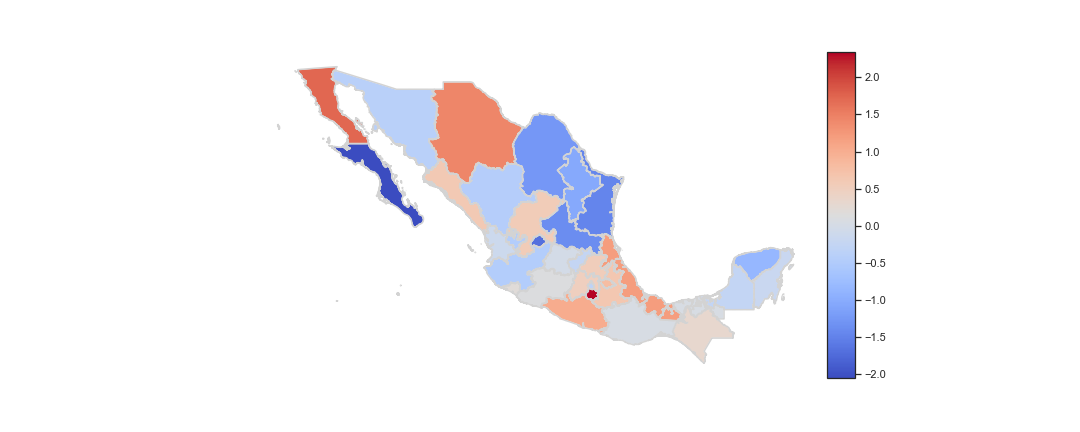
\includegraphics[width=1.1\linewidth]{map_risk_deaths}
		\caption{Deaths}
		\label{fig:sub1}
	\end{subfigure}%
	\begin{subfigure}{.5\textwidth}
		\centering
		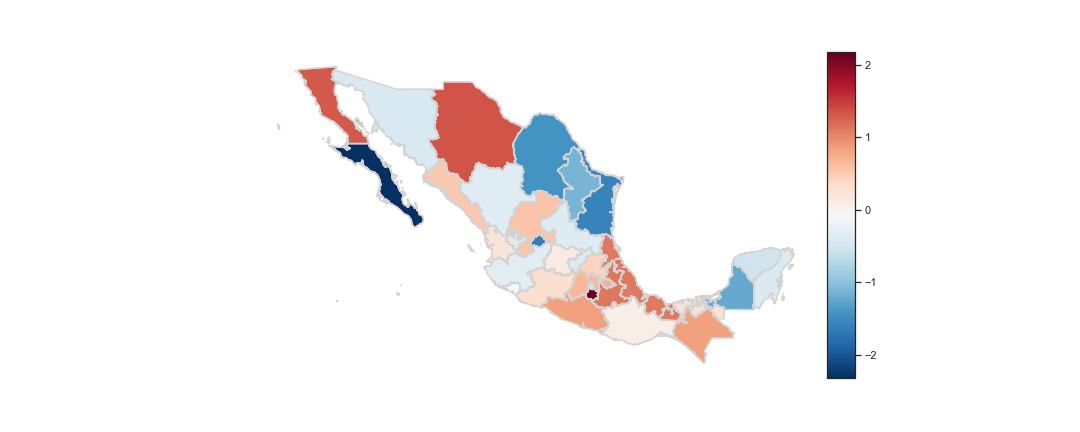
\includegraphics[width=1.1\linewidth]{map_risk_hosp}
		\caption{Hospitalizations}
		\label{fig:sub2}
	\end{subfigure}
	\caption{Relative Risk by State}
	\label{fig:test}
\end{figure}
	%%%%%%%%%%%%%%%%%%%%%%%%%

	\section{Policy Recommendations}\label{sec_pol}
	To delay the spread of COVID-19, Mexico’s government declared a health emergency and implemented a range of broad measures such as travel restrictions, social distancing, closure of schools, and shutdown of non-essential activities\footnote{\href{https://www.imf.org/en/Topics/imf-and-covid19/Policy-Responses-to-COVID-19\#M}{\textit{Policy Responses to COVID: Mexico.}}- International Monetary Fund}. However, these restrictions weren't fully enforced and there was non-compliance with social distancing and quarantine rules across Mexico, especially in the informal sector where people live on a daily income\footnote{\href{https://www.infobae.com/america/mexico/2020/04/19/en-la-periferia-de-ciudad-de-mexico-la-cuarentena-no-es-una-opcion/}{\textit{In Mexico City's periphery, quarantine is not an option.}}- Infobae}. During the first days of June, confirmed cases grew to 120,000 with more than 11\% confirmed deaths. Additionally, resources are highly limited particularly because the government refused to deviate from its “Fiscal Austerity” and to take on debt even when the country is facing a severe health and economic crisis.\\
	In this context, timely and efficient responses of the government to allocate scarce resources are imperative to face the current pandemic. Regional authorities could take a similar approach to ours and predict if an individual who tested positive for COVID-19 is likely to develop a severe case of the disease to focus resources on those vulnerable individuals. Moreover, targeted policies towards vulnerable communities can help mitigate the associated social and economic losses. Health aid, especially, preventive care resources (i.e tests, masks, sanitation products) and social isolation should be targeted towards the communities whose population is at risk of ending up in critical conditions if infected. In this report, we found that some features such as age and diabetes showed higher importance in predicting these outcomes. Hence, some policies could target older groups or groups that show a higher presence of comorbidities such as diabetes. Note that other studies (as Jiang, et al. 2020) that also predict severity in a COVID-patient show that age or diabetes are not as strong predictors as biochemical features (e.g. alanine aminotransferase, hemoglobin levels)
	Based on the risk index of this study, Baja California, Chihuahua, Sinaloa, Guerrero,  Veracruz, and Morelos are some of the states that have a relatively higher risk compared to the average level of risk in the country. This could be a starting point to further evaluate and identify vulnerable communities in Mexico in order to develop targeted policies that could prevent deaths and hospitalizations. However, we strongly advise the reader to take with caution when interpreting the risk index, as it was built on incomplete information (unreported COVID-19 cases and information by Mexican officials). Also, allocating scarce health resources can have ethical implications as we will discuss in the next section. 
	
	\section{Ethics}
	There are various ethical qualms that arise from our analysis.  To start, the main data set used documents of all official COVID-19 cases in Mexico and is, in all certainty, highly inaccurate. Furthermore, due to the lack of testing on certain rural regions in the country, we are also concerned that our analysis has ignored or failed to learn statistical relationships from  many vulnerable communities that are not recorded (or under-reported) in our data. \\To address this we visualized F1-score and recall-score across Mexico to illustrate how these evaluation metrics changed as a function of geography (Supplementary Figure~\ref{fig:9}). The differences in evaluation metrics that our models achieve as a function of geography are notable for both prediction outcomes (deaths and hospitalizations). Additionally, we are concerned about the possibility that the results of our analysis can be misinterpreted and lead to ill-informed excuses to stigmatize certain groups in the population. We implore any reader of our work to not make grandiose conclusions or extrapolate erroneous relationships. The purpose of our work is \textbf{NOT} to find causal relationships between health/socioeconomic variables and severe outcomes. Rather, our work helps to identify variables that might be indicative of which individuals are most vulnerable to the virus once infected. This allows policymakers and medical practitioners to prioritize these vulnerable individuals during the triage process and thus offer them the best care possible. \\
	Given that medical resources are finite and in many situations, as happened in the hardest hit areas of Lombardy and New York City, insufficient for all patients. Prioritizing certain individuals for care necessarily puts others at higher risk. We offer one possible framework to determine how to deal with this issue  by allocating resources to those which data suggest might have more complications (older individuals and individuals with comorbidities). Nonetheless, fair allocation of resources requires a multifaceted ethical framework that should reflect the resources, priorities and values of individual populations.
	
	\section{Limitations, Caveats, and Suggestions for Future Work}
	The main caveat to consider in this analysis, as mentioned before, is that the official data set for COVID-19 cases in Mexico that we used is, in all certainty, highly inaccurate.
	As has been discussed, Mexico’s testing capacity lags far behind many of its peers which means the official case count of infections used in this analysis is much smaller than the real number. Furthermore, it has been suggested that official statistics have underreported the number of deaths as a consequence of the virus\footnote{\href{https://www.nytimes.com/2020/05/08/world/americas/mexico-coronavirus-count.html}{\textit{Hidden Toll: Mexico Ignores Wave of Coronavirus Deaths in Capital.}}- Azam Ahmed. May 2020. The New York Times.}. Due to these inaccuracies, the results of our analysis are probably biased. Particularly, we only observe severe cases in the data, since in Mexico (as in many places in the world) only people with harsh symptoms are tested, due to the government reticence for performing mass-testing\footnote{\href{https://www.cnn.com/2020/05/15/americas/mexico-coronavirus-testing-intl/index.html}{\textit{Mass testing won't happen in Mexico. That's the way the government wants it.}}- Matt Rivers. May 2020. CNN.}. Additionally the data set provides very limited information on each individual; having more features could improve the models predictive power. Specifically, direct biochemical measurements such as glucose level, hemoglobin counts, etc.\\
	Regarding the Health Resources data, it's important to notice that this dataset only accounts for federally-funded health facilities; while we're missing data on state, municipal and privately funded hospitals, according to CONEVAL, more than 90\% of the reported COVID-19 cases are treated in federally-funded facilities\footnote{\href{https://www.coneval.org.mx/Medicion/MP/Paginas/Hallazgos\_Visor.aspx}{\textit{ Poverty and COVID-19 Findings}- CONEVAL}}.

	
	%%%%%%%%%%%%%%%%%%%%%%%%%
	\newpage
	\section{Additional References}\label{sec_ref}
	\begin{itemize}
		\item Caruana, R.; Lou, Y.; Gehrke, J.; Koch, P.; Sturm, M. et al. (2015): Intelligible models for healthcare: predicting pneumonia risk and hospital 30-day readmission. Proceedings of the 21th ACM SIGKDD International Conference on Knowledge Discovery and Data Mining, pp. 1721-1730.
		\item Chen, C., Liaw, A., \& Breiman, L. (2004). Using random forest to learn imbalanced data. University of California, Berkeley, 110(1-12), 24.
		\item Jiang, X., Coffee, M., Bari, A., Wang, J., Jiang, X. et al. (2020). Towards an Artificial Intelligence Framework for Data-Driven Prediction of Coronavirus Clinical Severity. CMC-Computers, Materials \& Continua, 63(1), 537–551.
			\item King, G., \& Zeng, L. (2001). Logistic regression in rare events data. Political analysis, 9(2), 137-163.
		\item Shipe, M. E., Deppen, S. A., Farjah, F., \& Grogan, E. L. (2019). Developing prediction models for clinical use using logistic regression: an overview. Journal of thoracic disease, 11(Suppl 4), S574.
		\item Vieira, S. Mendonça, L., Farinha, G., Sousa, J. (2013) Modified binary PSO for feature selection using SVM applied to mortality prediction of septic patients. Applied Soft Computing.
	
		
		
	\end{itemize}
\newpage 
\section{Appendix}
This study uses different machine learning models to predict the target variables (i.e. deaths and hospitalizations). 
\\
\\
Logistic regression is an extension of linear regression whose target prediction is binary. Unlike linear regression which assumes that the data follows a linear function, Logistic regression models the data using the sigmoid function. The function maps any real value into another value between 0 and 1. Logistic regression becomes a classification technique after choosing a decision threshold. 
\\
\\
Complement Naive Bayes is a Naive Bayes variant that estimates feature probabilities for each class based on its complement (i.e. on all other classes’ samples instead of on the training samples of that class itself). 
\\
\\
A SVM finds the best hyperplane that divides data points belonging to different classes in the test set. The name "Support Vector" comes from the fact that the algorithm will find observations in the training set (data points) that are equidistant from the hyperplane (or line in 2d). These support vectors determine which is the optimal hyperplane. Once the best hyperplane is found using the training set we can classify observations on the test set by observing on which side of the hyperplane they fall on.
\\
\\
Decision Trees predict the value of a target variable by learning simple decision rules inferred from the data features. Generally, these rules can be summarized in terms of a tree. Hence, these methods are called decision tree methods. 
\\
\\
A Random Forest algorithm creates decision trees on data samples and then gets the prediction from each of them and finally selects the best solution by means of voting. This method is better than a single decision tree because it reduces the over-fitting by averaging the result.


	\newpage
	\subsection{Supplementary Figures}\label{sec_app}
	\setcounter{figure}{0} 
		\begin{figure}[ht!]
		\caption{Total COVID-19 reported cases in Mexico}
		\centering 
		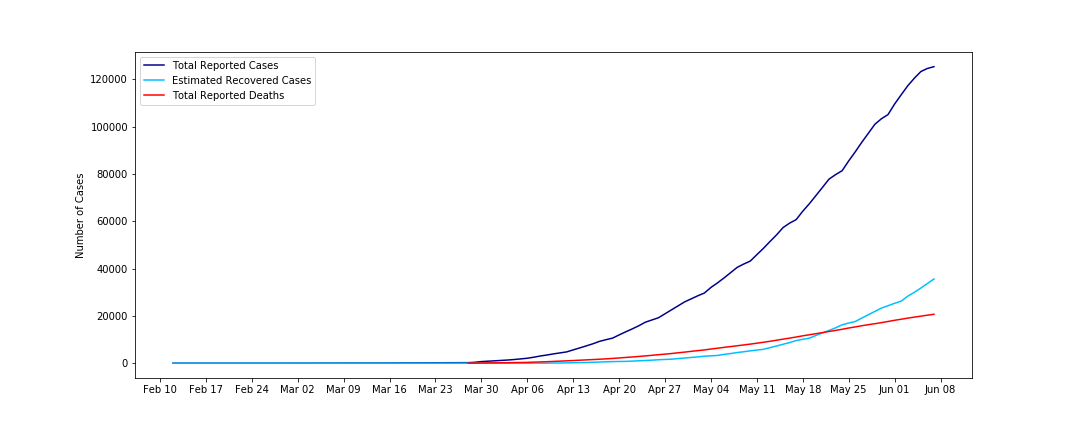
\includegraphics[width=0.97\textwidth]{Total_Cases}
		\floatfoot{Source: Health Ministry data}
		\label{fig:1}
	\end{figure}
\begin{figure}[ht!]
	\caption{COVID-19 positive cases vs. deaths by state in Mexico}
	\centering 
	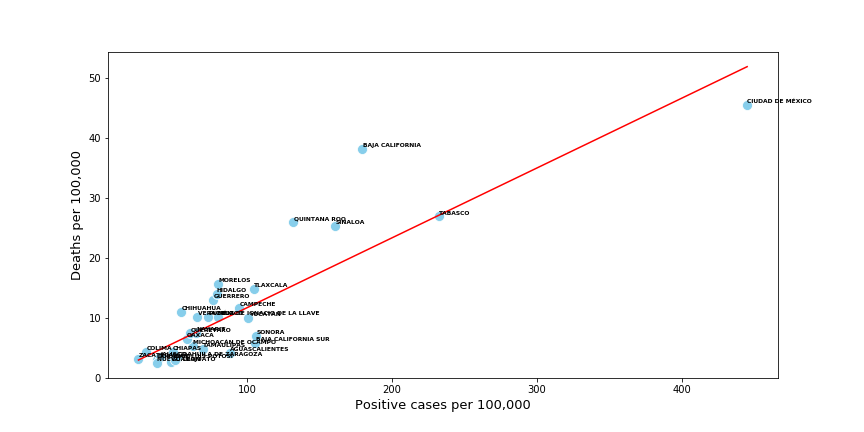
\includegraphics[width=0.97\textwidth]{CasesVSdeaths}
	\floatfoot{Source: Health Ministry data}
	\label{fig:2}
\end{figure} 
\begin{figure}[ht!]
	\caption{Age distribution for reported COVID-19 cases in Mexico}
	\centering 
	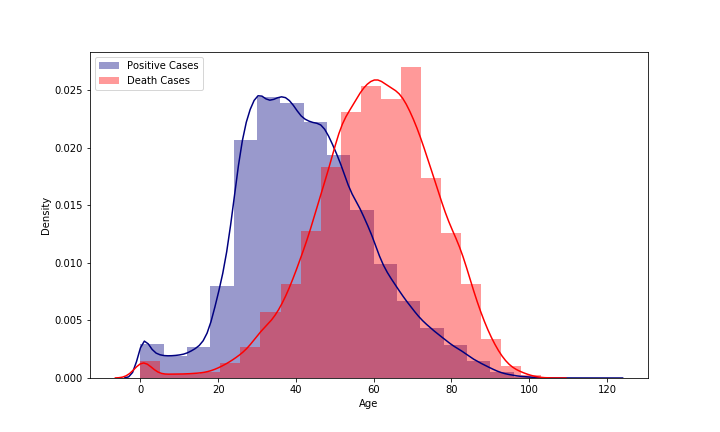
\includegraphics[width=0.8\textwidth]{Age_distribution}
	\floatfoot{Source: Health Ministry data}
	\label{fig:3}
\end{figure} 
	\begin{figure}[ht]
	\caption{COVID-19 Daily New Cases, Hospitalizations and Deaths in Mexico}
	\centering 
	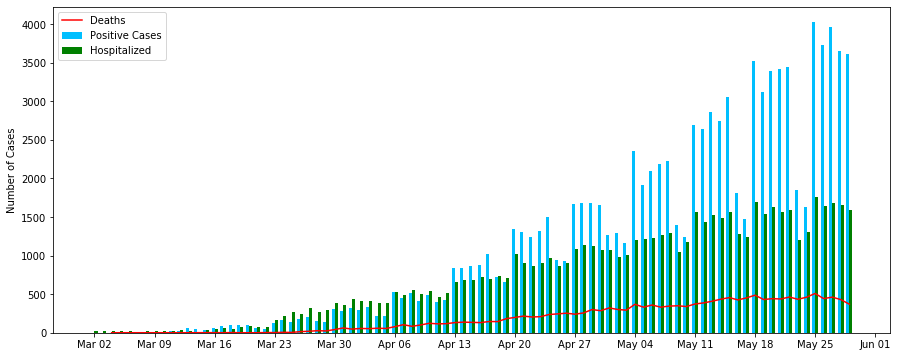
\includegraphics[width=0.9\textwidth]{output_5_0}
	\floatfoot{Source: Health Ministry data}
	\label{fig:4}
\end{figure}
\begin{figure}[ht]
	\caption{Data structure}
	\centering 
	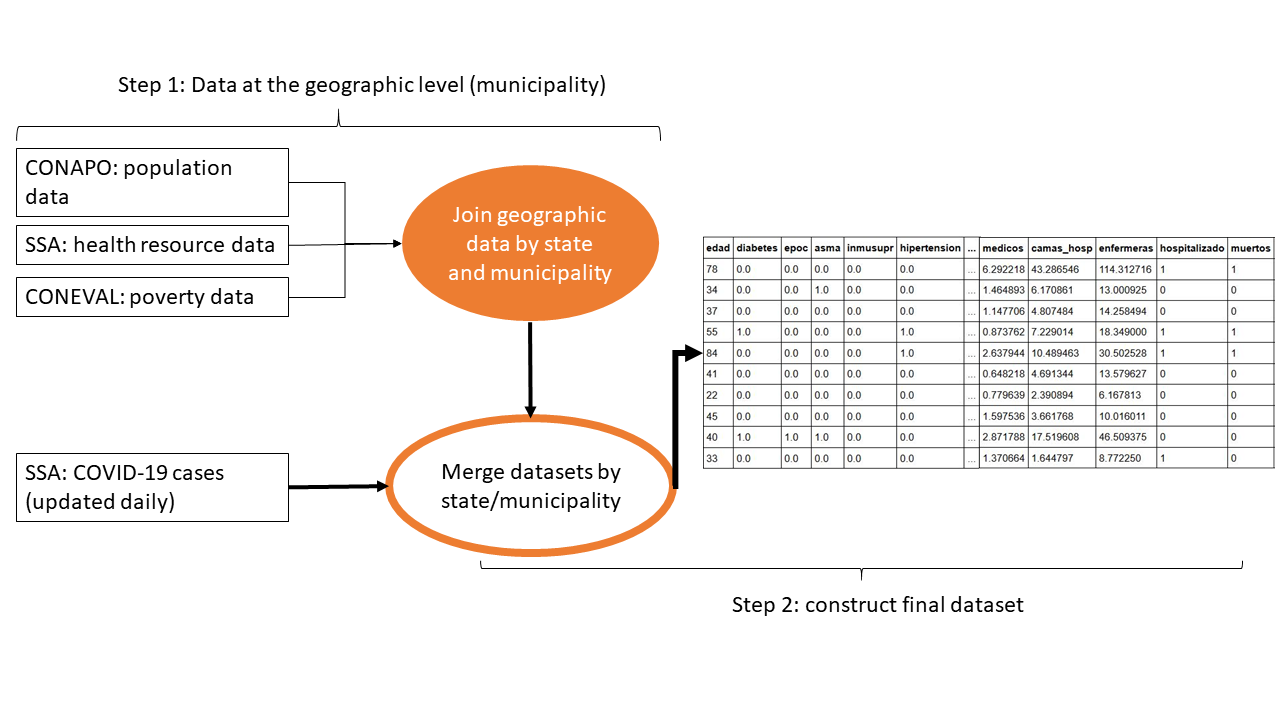
\includegraphics[width=0.9\textwidth]{FinalDF}
	\label{fig:5}
\end{figure}
\begin{figure}[ht]
	\caption{Cross-validation process}
	\centering 
	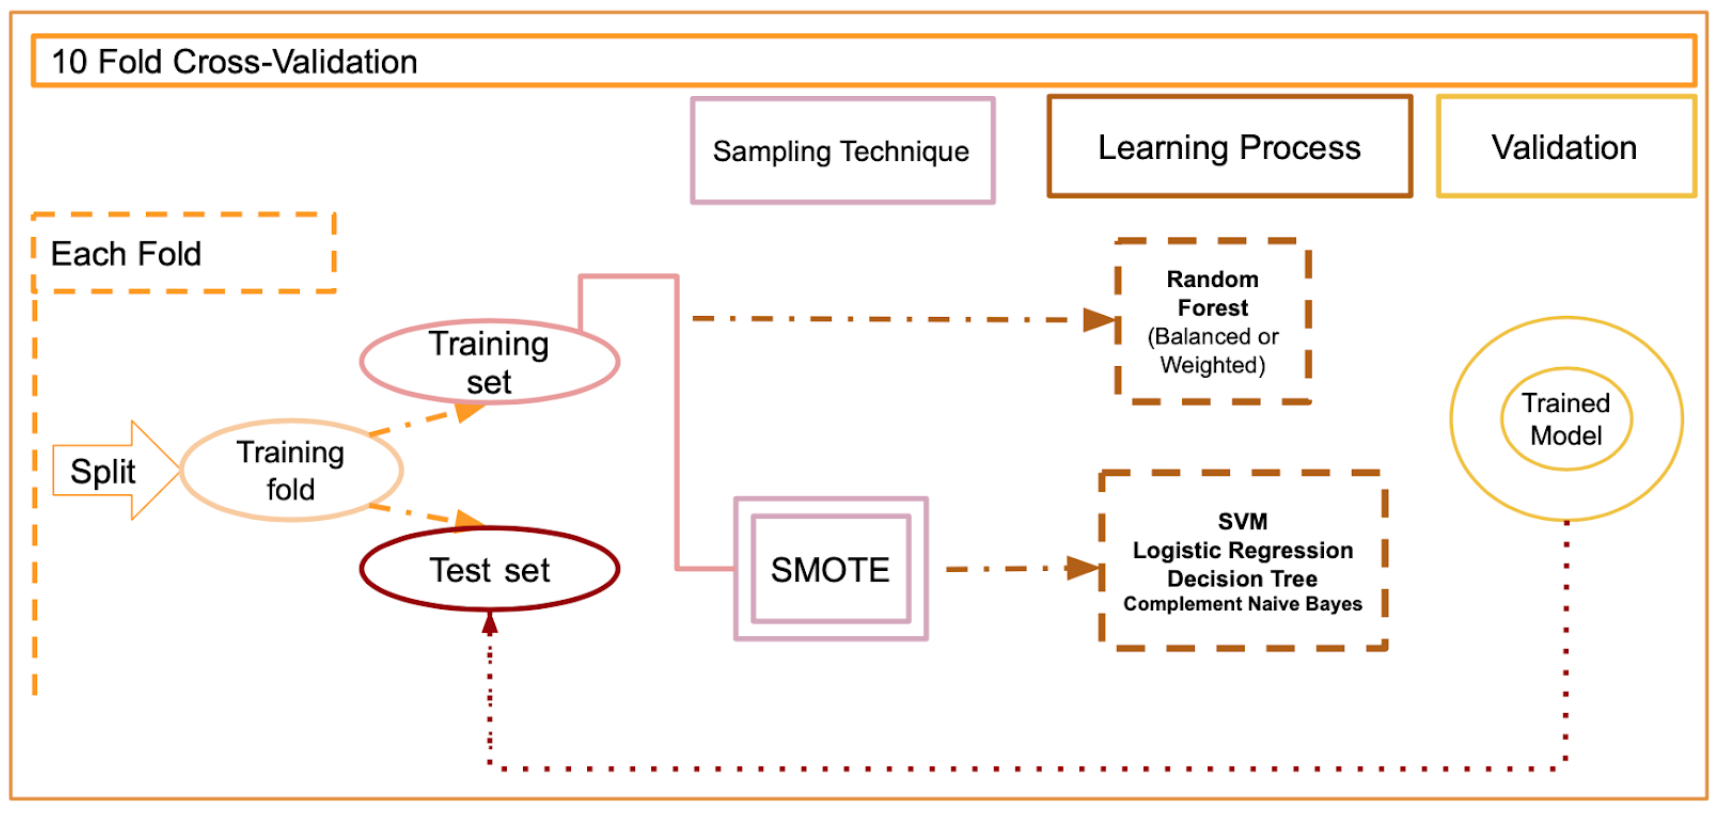
\includegraphics[width=0.9\textwidth]{cv}
	\label{fig:6}
\end{figure}

\begin{figure}[ht]
	\caption{Feature importance for COVID-19 deaths and hospitalizations prediction using SVM classifier }
	\centering
	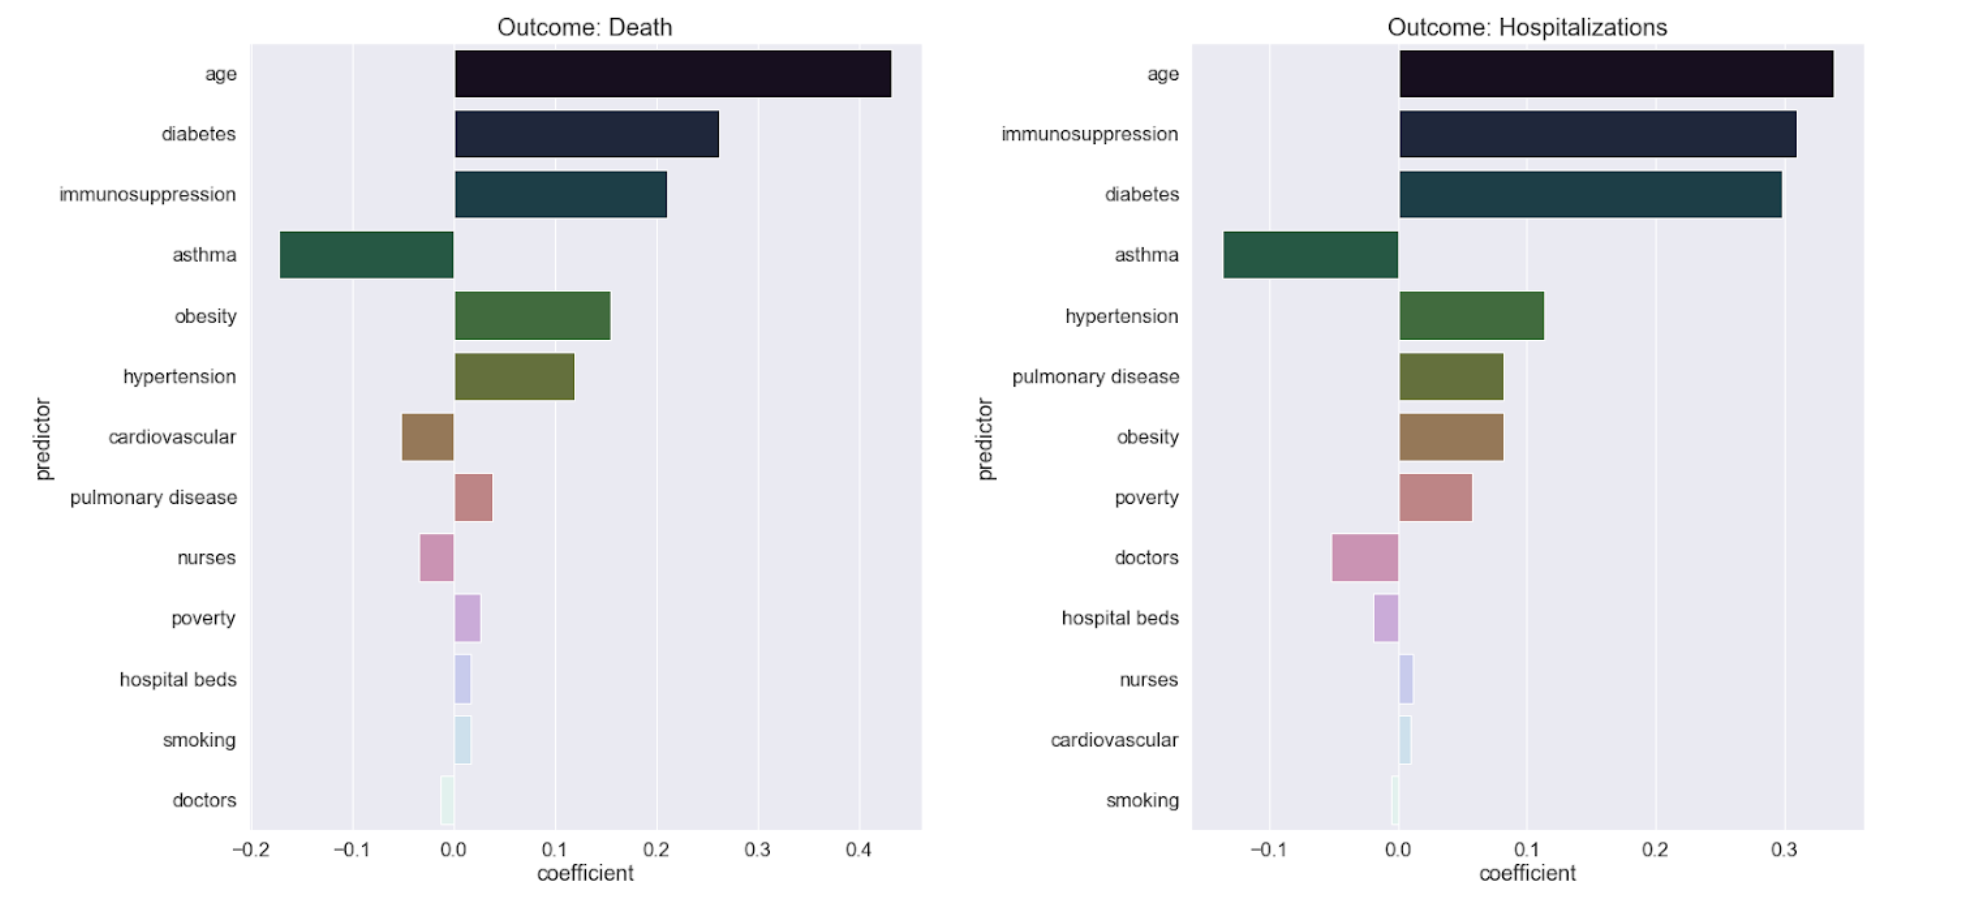
\includegraphics[width=0.95\textwidth]{feat1}
	\label{fig:7}
\end{figure}
\begin{figure}[ht]
	\caption{Feature importance for COVID-19 deaths and hospitalizations prediction using Random Forest classifier}
	\centering
	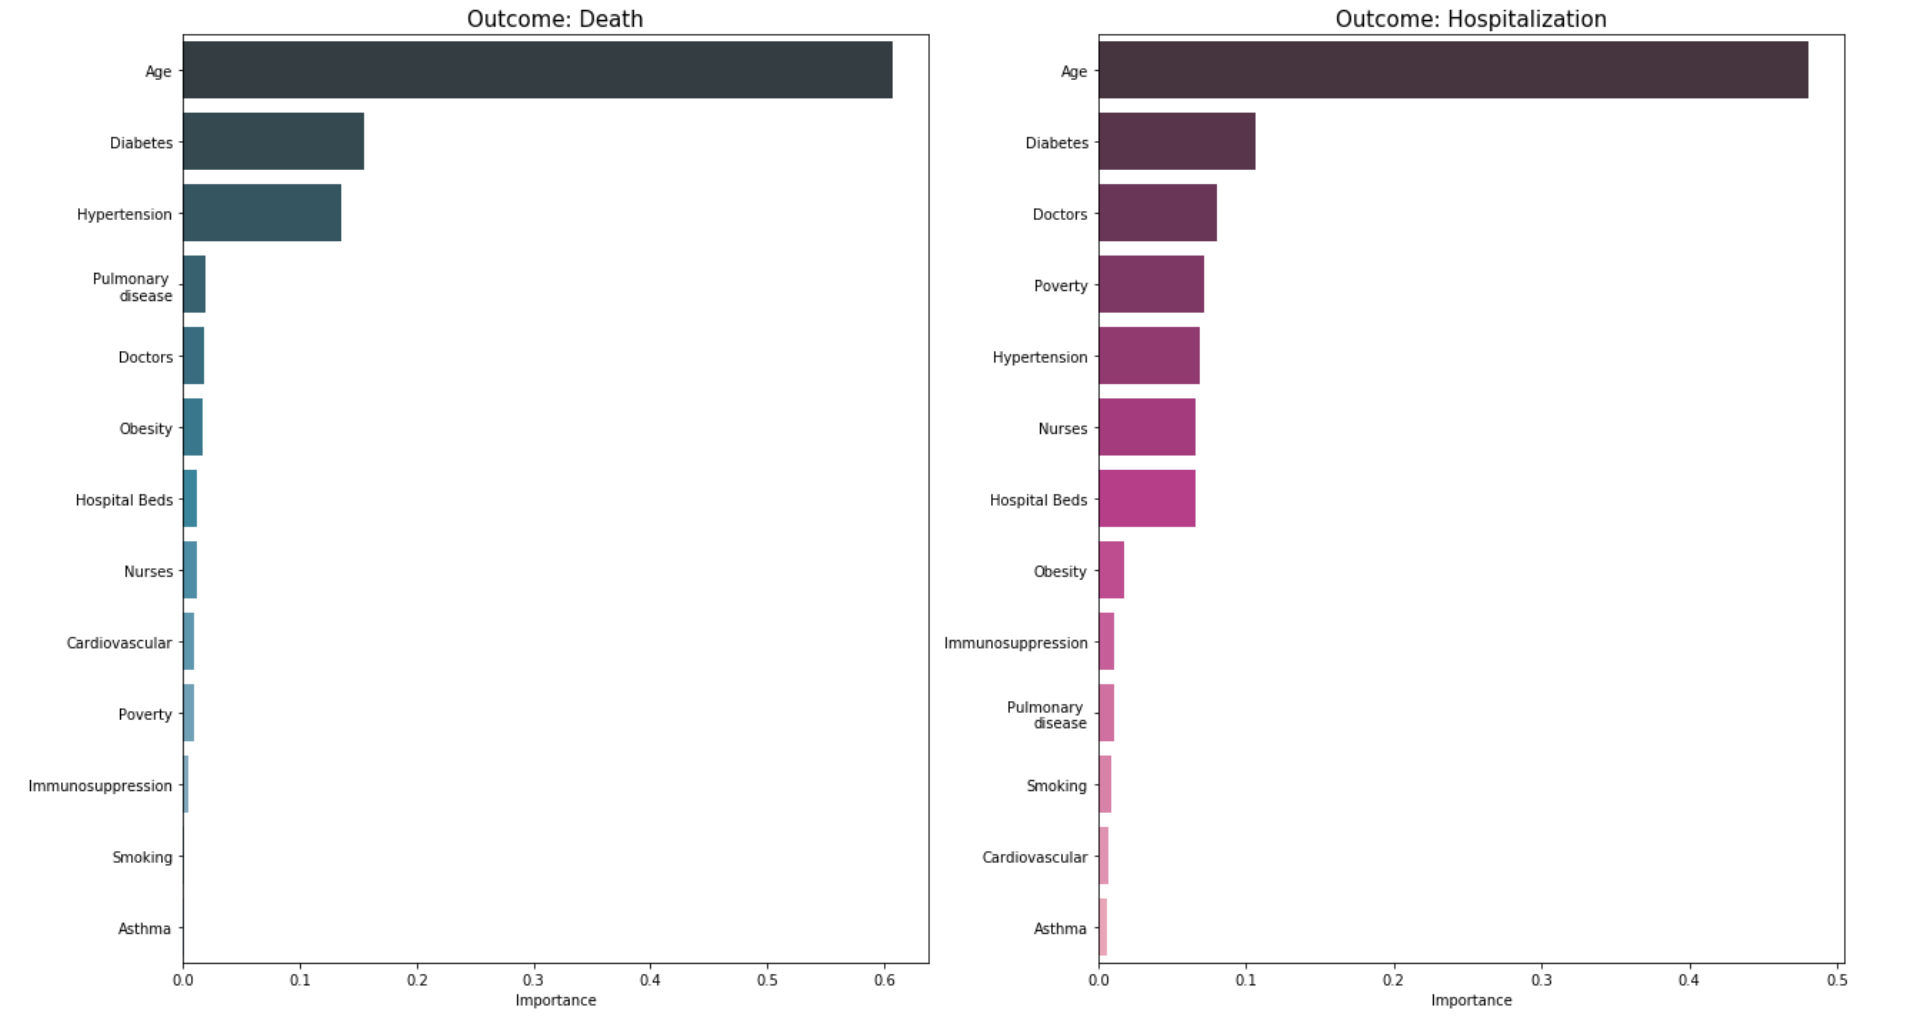
\includegraphics[width=0.85\textwidth]{feat2}
	\label{fig:8}
\end{figure}
	\begin{figure}[ht]
		\caption{Recall and F-1 scores for target variables by state}
		\centering 
		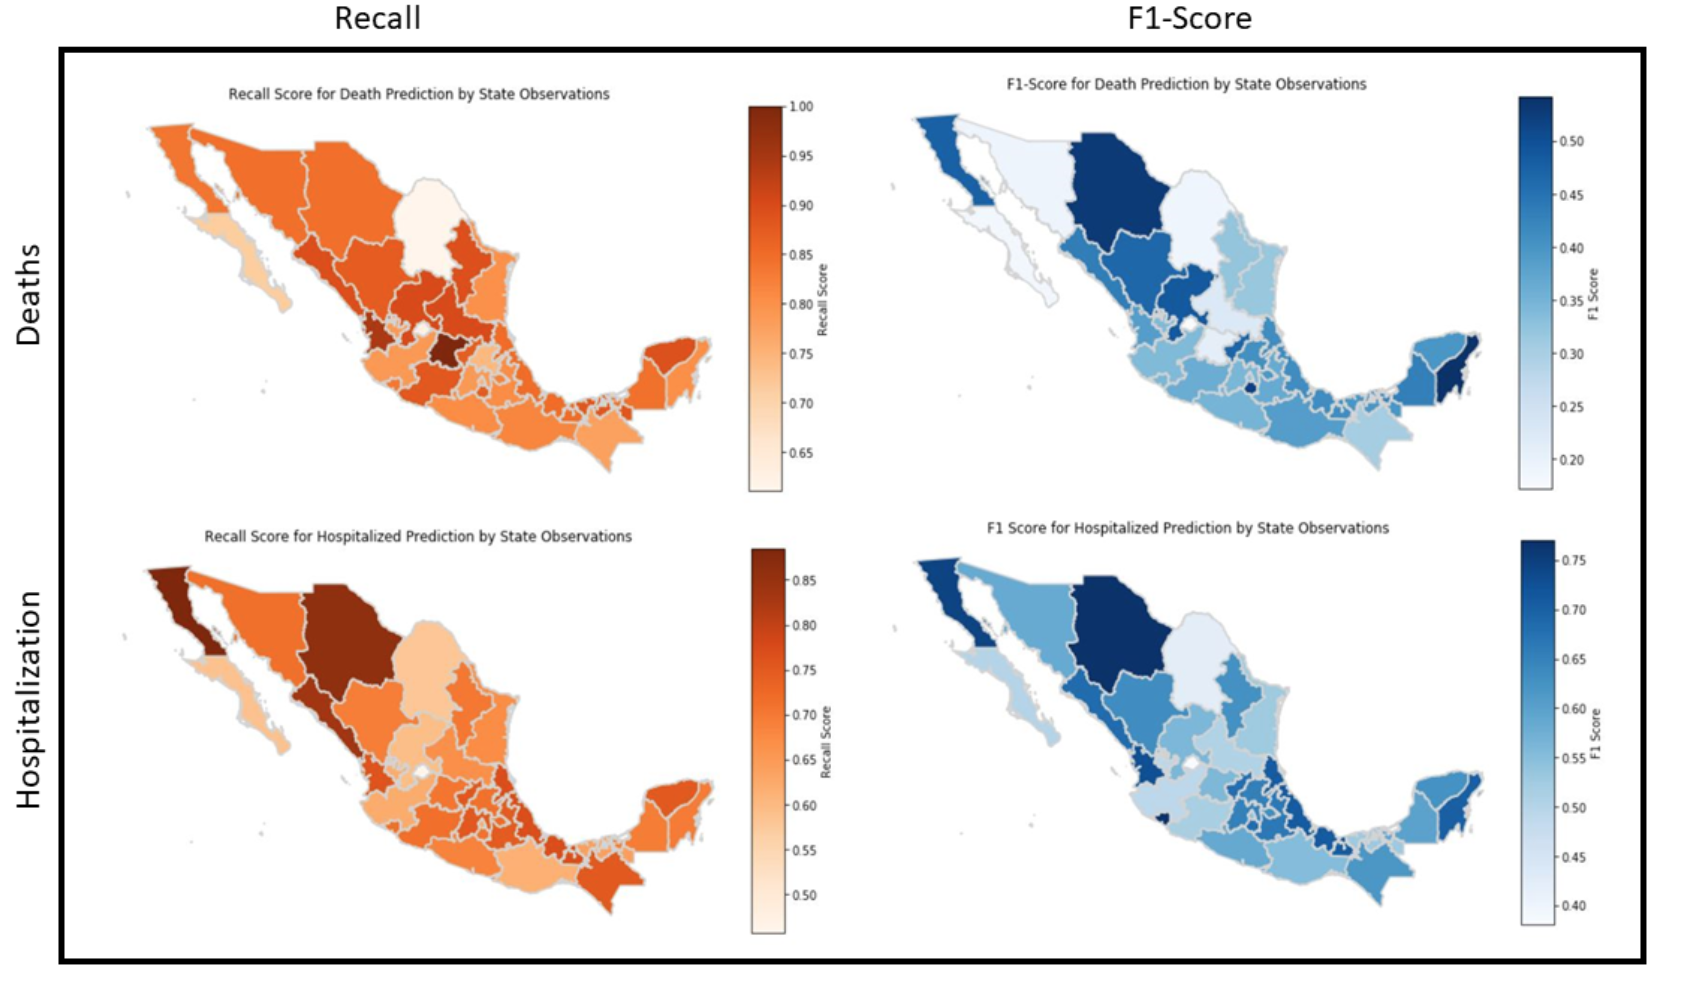
\includegraphics[width=0.9\textwidth]{f1}
		\label{fig:9}
	\end{figure}
	
	%%%%%%%%%%%%%%%%%%%%%%%%%
	
\end{document}